\chapter{Algoritmus}
\label{kap:algoritmus}
Po preskúmaní triangulačných algoritmov sme sa v našej práci rozhodli venovať čo najkvaitnejšiemu
prevedeniu triangulácie s menším dôrazom na rýchlosť výpočtu. Ako základnú štruktúru sme použili 
postup, ktorí uviedli autori článku \cite{hilton1996marching}. Tento algoritmus využíva 
\textit{Delaunayovu podmienku} predstavenú v kapitole \ref{kap:delaunay_triangulation}.
Daný algoritmus je implementovaný ako prechod cez frontu, v ktorej sa na úvod nachádzajú
hrany počiatočného trojuholníka, v každom kroku vyberieme z fronty jednu hranu $E$ a pre túto
hranu vykonáme nasledujúcu postupnosť krokov:
\begin{enumerate}
    \item{Vytvoríme vrchol $x_{proj}$ tak, ako sme opísali v kapitole \ref{kap:marching_triangles}, teda 
    ako bod ležiaci v kolmej vzdialenosti $k$ od stredu hrany $E = (x_i, x_j)$ 
    v rovine susedného trojuholníka $T$.}
    \item{Nájdeme vrchol $x_{new}$ ako vrchol, ktorý leží na povrchu a je blízko k bodu 
    $x_{proj}$. Tento bod projektujeme na plochu v smere $\nabla F(x_{proj})$.
    Platí teda, že $F(x_{new}) = 0$.}
    \item{Skončíme ak je splnená jedna z nasledujúcich možností:
    \begin{itemize}
        \item{Vrchol $x_{new}$ leží na hranici, teda medzi hraničnými 
        hranami sa nachádza hrana s vrcholom $x_{new}$.}
        \item{Normála $n_{new}$ trojuholníka $T_{new}$ ktorého vrcholy sú $x_i, 
        x_j, x_{new}$ je opačná ako
        normála $\overrightarrow{n}$ susedného trojuholníka $T$, teda 
        $\overrightarrow{n}_{new} \cdot \overrightarrow{n} < 0$.}
    \end{itemize}
    }
    \item{Pre trojuholník $T_{new}$ overíme platnosť \textit{Delaunayovej podmienky}, 
    ktorú sme predstavili v kapitole \ref{kap:delaunay_triangulation}, ak podmienka platí
    vykonáme nasledujúce kroky a prejdeme na ďalšiu hranu.
    \begin{itemize}
        \item{Pridáme vrchol $x_{new}$ do zoznamu vrcholov.}
        \item{Pridáme trojuholník $T_{new}$ do meshu.}
        \item{Pridáme hrany $(x_i, x_{new})$ a 
        $(x_j, x_{new})$ do fronty s hranami.}
    \end{itemize}
    }
    \item{
        Ak podmienka neplatí overíme platnosť \textit{Delaunayovej podmienky} pre Trojuholníky 
        $T_{prev}$, ktorého vrcholy sú $x_i, x_j, 
        x_{prev}$ a $T_{next}$, ktorého vrcholy sú 
        $x_i, x_j, x_{next}$, kde 
        $x_{prev}$ a $x_{next}$ sú hraničné vrcholy,
        pričom $x_{prev}$ 
        je sused vrchola $x_i$ a $x_{next}$ je sused vrchola 
        $x_j$. Ak niektorý z nich podmienku
        spĺňa, vykonáme preň body z kroku 4 a prejdeme na ďalšiu hranu.
    }
    \item{
        Ak všetky trojuholníky $T_{new}$, $T_{prev}$ ani $T_{next}$ nespĺňajú podmienku, potom 
        ak \textit{Delaunayova guľa} obsajuhe hraničný vrchol $x_{overlap}$ nejakého hraničného 
        trojuholníka $T_{overlap}$, ktorý je rovnako orientovaný ako hraničný trojuholník T, teda
        platí $n*n_{overlap} > 0$, potom overíme platnosť \textit{Delaunayovej podmienky} pre 
        trojuholník $T_{overlap}$ kde $x_{overlap}$ je najbližší k hrane E zo všetkých hraničných
        vrcholov, ktoré sa nachádzajú v Delaunayovej guli. Ak podmienku spĺňa aplikujeme naň body z 
        kroku 4 a prejdeme na ďalšiu hranu.
    }
    \item{
        Ak žiadny trojuholník nebol pridaný do meshu, testovanie hrany E skončíme.
    }
\end{enumerate}

Tento algoritmus používame v našej práci ako základnú štruktúru a pridávame do neho ďalšie podmienky 
a postupy na skvalitnenie výslednej triangulácie. V neadaptívnej verzií volíme vzdialenosť $k$ ako 
výšku rovnostranného trojuholníka so stranou dĺžky zadanej ako vstupný parameter algoritmu, teda 
$\frac{\sqrt{3}}{2}*strana$.

Náš algoritmus je z triedy \textit{Surface Tracking} algoritmov, teda algoritmus sledujúci povrch.
Funguje na princípe postupného pridávania trojuholníkov do rozpracovaného meshu. V každom kroku
pridávame najviac jeden trojuholník.

Na vstupe algoritmu sú nasledujúce dáta:
\begin{itemize}
    \item{
        Funkcia $F$ zadaná implicitne.

        Nulová hladina tejto funkcie určuje plochu, ktorú chceme triangulovať. 
        Zadaná plocha musí byť hladká, teda bez singularít.
    }
    \item{
        Veľkosť hrany $a$ trojuholníka.

        Toto je priližná veľkosť hrany trojuholíka v triangulácii. 
        Čím je veľkosť hrany menšia, tým je triagulácia presnejšia. Veľkosť hrany trojuholníka 
        nesmie byť príliš však príliš veľká. Malá veľkosť hrany zvyčajne nevadí, avšak pre 
        menšie trojuholníky trvá algoritmus omnoho dlhšie.
    }
    \item{
        Počiatočný bod $x_{seed}$ v ktorom začneme trianguáciu povrchu. 

        Tento bod musí ležať na povrchu alebo dostatočne blízko na povrchu.
    }
    \item{
        Ohraničenie.

        Pre ohraničenú trianguláciu potrebujeme zadať hranicu ohraničenia. Pre každú z troch súradníc 
        sú to 2 čísla - minimum a maximum, teda spolu 6 čísel.
    }
\end{itemize}

Začneme vytvorením jediného trojuholníka s veľkosťou hrany približle $a$, presný spôsob implementácie
opíšeme v kapitole TODO.

Funkčnosť algoritmu opíšeme akosi indukčne. Majme korektnú čiastočnú trianguáciu povrchu, na začiatku
je to jediný trojuholník. Prvá otázka ktorú si pokladáme je nasledujúca. 
\textit{Aké podmienky musí spĺňať trojica vrcholov} $x_i, x_j, x_k$ 
\textit{aby sme ju pridali do triangulácie ako nový trojuholník na hraničnej hrane} $E = (x_i, x_j)?$ 

\section{Pridanie trojuholníka do meshu}
\label{kap:triangle_conditions}

Majme hraničnú hranu $E=(x_i, x_j)$ čiastočnej triangulácie $M$ a bod $x_k \in \mathbb{E}^3$. 
Tento bod sa môže aj nemusí nachádzať medzi vrcholmi $M$. Za akých podmienok môžeme pridať trojuholník 
$T=(x_i, x_j, x_k)$ do $M$?

\begin{enumerate}
    \item{
        \textit{Trojica bodov tvorí trojuholník.}


        Veľmi zjavná avšak veľmi dôležitá podmienka. Ak by sme však overovali klasickú 
        \textit{trojuholníkovú nerovnosť} vyradili by sme iba kolineárne trojice bodov. My však nechceme 
        umožniť ani tvorbu extrémne úzkych trojuholníkov, preto upravíme podmienku aby vyradila aj tieto
        trojuholníky a to tak, že súčet dĺžok každej dvojice strán musí byť väčší od dĺžky tretej aspoň
        o nejakú malú konštantu $z$.
    } 

    \item{
        \textit{Trojuholník je správne orientovaný.}


        Čo znamená správna orientácia môžeme vidieť na obrázku \ref{obr:good_orientation}. Uhol $\beta$
        počítame ako uhol dvoch vektorov $\overrightarrow{x_i x_j}$ a $\overrightarrow{x_i x_{new}}$, 
        pričom nás zaujíma nie len veľkosť uhla ale aj orientácia vzhľadom na susedný trojuholník. To 
        vyjadríme znamienkom pri veľkosti uhla. 

        \begin{figure}
            \centerline{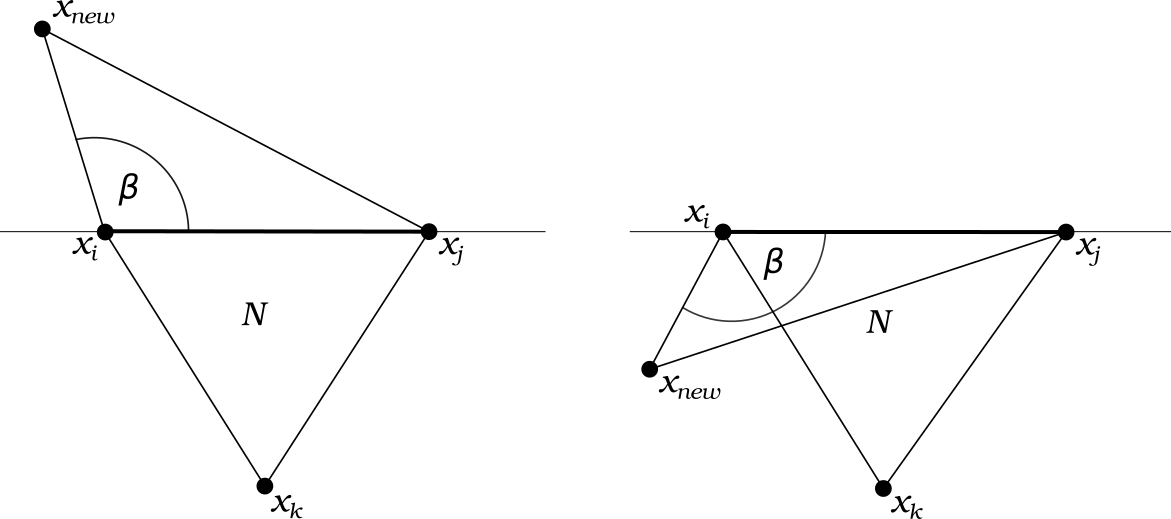
\includegraphics[width=0.55\textwidth]{images/good_orientation}}
            \caption[]{$T(x_i, x_j, x_{new})$ \textit{naľavo} má správnu orientáciu, \textit{napravo} má nesprávnu.}
            %id obrazku, pomocou ktoreho sa budeme na obrazok odvolavat
            \label{obr:good_orientation}
        \end{figure}

        Pod orientáciou vzhľadom na susedný trojuholník myslíme nasledovné.
        Ak

        $$(\overrightarrow{x_i x_j} \times \overrightarrow{x_i x_k}) 
        \cdot (\overrightarrow{x_i x_j} \times \overrightarrow{x_i x_{new}}) < 0$$

        tak je uhol v intervale $(0, \pi)$, inak je uhol v intervale $<-\pi, 0>$.
        
        Intuícia za predchádzajúcim vzťahom je taká, že vektorový súčin 
        $\overrightarrow{x_i x_j} \times \overrightarrow{x_i x_k}$ ukazuje \textit{do obrazovky}.
        Vektorový súčin $\overrightarrow{x_i x_j} \times \overrightarrow{x_i x_{new}}$ ukazuje 
        \textit{von z obrazovky} v prípade naľavo, avšak \textit{do obrazovky} v prípade napravo.
        Skalárny súčin týchto smerov je kladný práve vtedy, keď ukazujú \textit{tým istým smerom}, 
        teda ich uhol je menej ako $\frac{\pi}{2}$. 
        
        Trojuholník má \textit{správnu orientáciu} vzhľadom
        na susedný trojuholník $N$, práve vtedy keď uhol $\beta \in (0, \pi)$. V našej implementácii 
        však nechceme príliš úzke trojuholníky, túto podmienku sme teda upravili na podmienku
        $\beta \in (\frac{\pi}{10}, \frac{9\pi}{10})$. Vizualizáciu oblasti, z ktorej sú vhodné 
        vrcholy pre trojuholník $T$ a jeho hraničnú hranu $E$ môžeme vidieť na obrázku 
        \ref{obr:good_orientation_points}.

        \begin{figure}
            \centerline{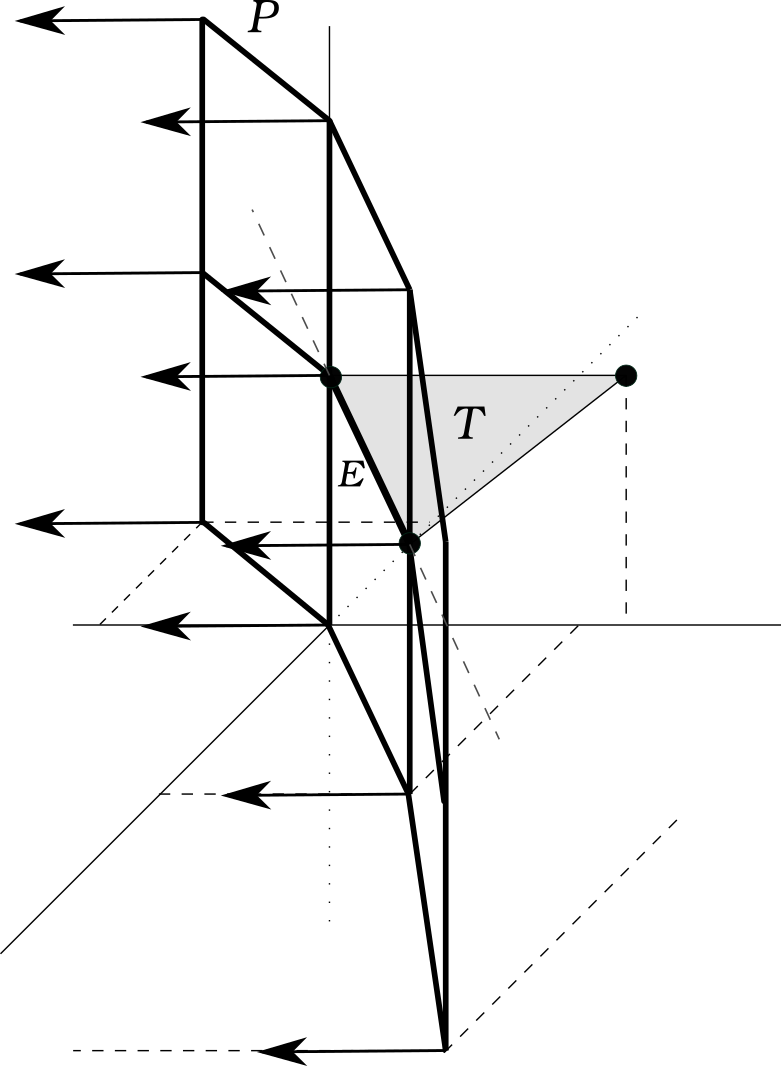
\includegraphics[width=0.25\textwidth]{images/good_orientation_points}}
            \caption[]{Vyhovujúce body sa nachádzajú \textit{naľavo} od plochy $P$.}
            %id obrazku, pomocou ktoreho sa budeme na obrazok odvolavat
            \label{obr:good_orientation_points}
        \end{figure}

        Oblasti, v ktorých by sme pri triangulácii potrebovali aby mali susedné 
        trojuholníky uhol normál väčší ako $\frac{\pi}{2}$ sú oblasti s veľkým zakrivením. 
        V týchto oblastich musíme buď zmenšiť veľkosť hrany trojuholníka
        pre celý model alebo v adaptívnej verzii v takýchto oblastiach 
        prispôsobiť veľkosť trojuholníkov. 
    }

     \item{
         \textit{Pre nové hrany $(x_i, x_{new})$ a $(x_j, x_{new})$ platí jedna z nasledujúcich podmienok
         \begin{enumerate}
            \item {
                Hrana je \textit{nová}, teda sa nenachádza medzi doterajšími hranami meshu. 
            }
            \item {
                Ak sa hrana nachádza v meshi, tak je \textit{hraničná}.
            }
         \end{enumerate}
         }
     }

     \item{
         \textit{Pre trojuholník je splnená \textit{Delaunayova podmienka} tak, ako bola opísaná v 
         definícii \ref{def:delaunay_constraint}.}

        Ako neskôr uvidíme, túto podmienku nemusia nutne spĺňať všetky trojuholníky. Náš algoritmus sa bude 
        skladať z dvoch častí, v prvej časti vyžadujeme od všetkých trojuholníkov splnenie tejto podmienky.
        Po skončení prvej časti zostávajú v meshi diery, ktoré je možné vyplniť trojuholníkmi nespĺňajúcimi 
        \textit{Delaunayovu podmienku}. Príklad takejto diery môžeme vidieť na obrázku 
        \ref{obr:non_delaunay_triangle}. Hrubšie hrany vyjadrujú hraničné hrany triangulácie. 
        Vidíme, že by sme chceli vytvoriť trojuholník $T = (x_i, x_j, x_k)$,
        avšak tento trojuholník nespĺňa \textit{Delaunayovu podmienku}. Takéto trojuholníky
        budeme riešiť v druhej časti algoritmu.
     }

     \item{
         \textit{V okolí bodu $x_{new}$ sa nenachádza ťažisko už existujúceho trojuholníka.}

         Táto podmienka, tak isto ako \textit{Delaunayova podmienka}, nebude musieť byť splnená vždy,
         avšak taktiež ju vyžadujeme v prvej časti algoritmu. 
         
         Túto podmienku sme zvolili preto, že vo veľkej miere eliminuje problémy s pretínaním 
         trojuholníkov ak overujeme Delaunayovu podmienky iba pre trojuholník, ktorý chceme pridať 
         avšak nie pre všetky trojuholníky meshe. Tento problém si všimli aj autori S. Akkouche a 
         E. Gallin \cite{akkouche2001adaptive}, ktorí navrhli ako riešenie pri pridávaní trojuholníka 
         overovať \textit{Delaunayovu podmienku} aj pre už existujúce trojuholníky. 
         
         Tento prístup sme otestovali a myslíme si, že je príliš prísny a zbytočne odmieta aj trojuholníky, 
         ktoré sa nám zdajú vhodné. Navyše vznikajú pomerne rozsiahle diery, ktoré sa nie vždy podarí 
         vhodne opraviť, keďže v časti algoritmu pre opravovanie dier sa už neoveruje
         \textit{Delaunayova podmienka}.

         Ťažisko trojuholníka sme ako oporný bod zvolili z viacerých dôvodov.
         \begin{itemize}
            \item{
                \textit{Je vždy vnútri trojuholíka.}

                Hlavný problém, prečo overovanie Delaunayovej podmienky pre všetky trojuholníky spôsobuje
                odmietanie aj vhodných trojuholníkov je ten, že stred opísanej kružnice nemusí byť vždy
                vnútri trojuholníka. Čím je trojuholník užší, tým je dokonca vzdialenejší a tak môže aj
                vzdialenejší úzky trojuholník spôsobiť nevzniknutie vhodného trojuholníka. 
            }
            \item{
                \textit{Lepšie vystihuje polohu trojuholníka.}

                Ak chceme zabrániť tvorbe prekrývajúcich sa trojuholníkov je pre nás dôležité zaujímať sa 
                o polohu ostatných trojuholníkov v meshi. Ťažisko sa nám zdá ako najvhodnejší bod na 
                vystihnutie tejto polohy.
            }
            \item{
                \textit{Vieme ho jednoducho vypočítať.}

                Mohli by sme počítať aj priamo pretínanie trojuholníkov, to je však v $3D$ pomerne 
                výpočtovo náročný proces, kdežto ťažisko trojuholníka a takisto jeho vzdialenosť od 
                bodu vieme vypočítať veľmi jednoducho.
            }
         \end{itemize}
         
         \begin{figure}
         \centerline{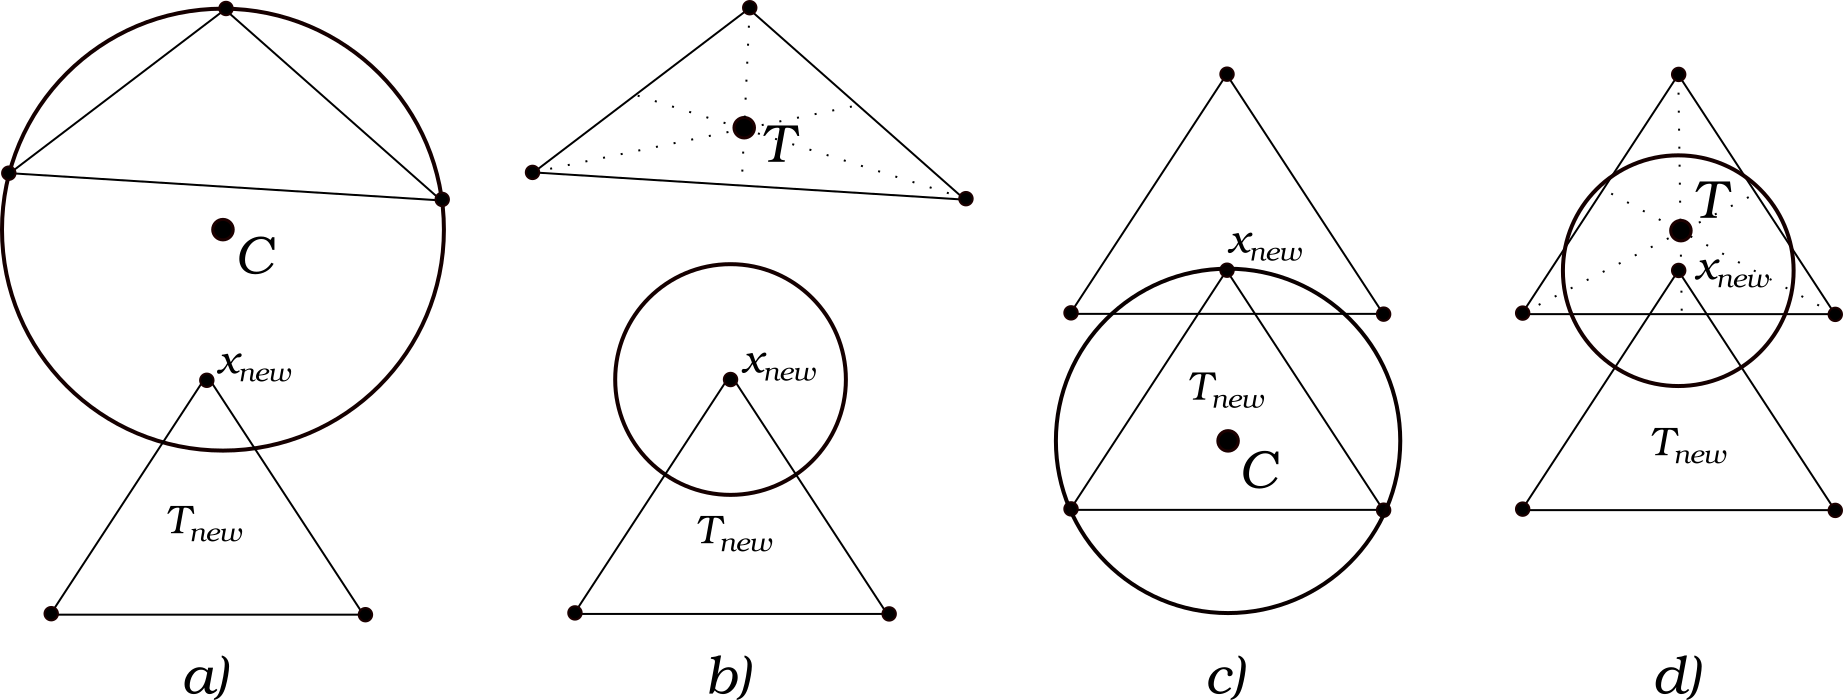
\includegraphics[width=0.8\textwidth]{images/delaunay_vs_gravitycenter_2}}
         \caption[]{TODO}
         %id obrazku, pomocou ktoreho sa budeme na obrazok odvolavat
         \label{obr:delaunay_vs_gravitycenter_2}
         \end{figure}
         
         Na obrázku \ref{obr:delaunay_vs_gravitycenter_2} môžeme vidieť:
         \begin{enumerate}[a)]
            \item{
                Nový vrchol $x_{new}$ nespĺňa Delaunayovu podmienku už existujúceho trojuholníka aj 
                napriek tomu, že trojuholník $T_{new}$ môžeme bez problémov môžeme vytvoriť a 
                neporušíme konzistenciu triangulácie.
            }
            \item{
                Nový vrchol $x_{new}$ spĺňa podmienku a môžeme pridať trojuholník $T_{new}$ do meshu.
            }
            \item{
                Trojuholník $T_{new}$ spĺňa \textit{Delaunayovu podmienku} popísanú v definícii 
                \ref{def:delaunay_constraint} avšak prekrýva sa s už existujúcim trojuholníkom.
            }
            \item{
                Nový vrchol $x_{new}$ sa nachádza v blízkosti ťažiska existujúceho trojuholníka, 
                teda trojuholník $T_{new}$ nespĺňa našu podmienku a do meshu ho nepridáme. 
            }
         \end{enumerate}


         Na obrázku \ref{obr:delaunay_vs_gravitycenter} môžeme vidieť ten 
         istý algoritmus s rovnakými parametrami spustený bez časti, ktorá uzatvára diery. 
         
         Naľavo vidíme výsledok dosiahnutý pri prístupe, ktorý v \textit{Delaunayovej podmienke} overuje aj
         Delaunayovu podmienku ostatných trojuholníkov. 
         
         Napravo vidíme výsledok, ktorý v Delaunayovej
         podmienke overuje blízkosť ťažiska ostatných trojuholníkov. Napriek tomu, že algoritmus
         je v oboch prípadoch spustený bez časti ktorá uzatvára diery v druhom prípade je výsledná 
         triangulácia bez dier, avšak vo veľkej väčšine prípadov eliminuje problémy, ktoré vznikali 
         pri overovaní \textit{Delaunayovej podmienky} iba pre trojuholník, ktorý pridávame.
     }

    \begin{figure}
        \centerline{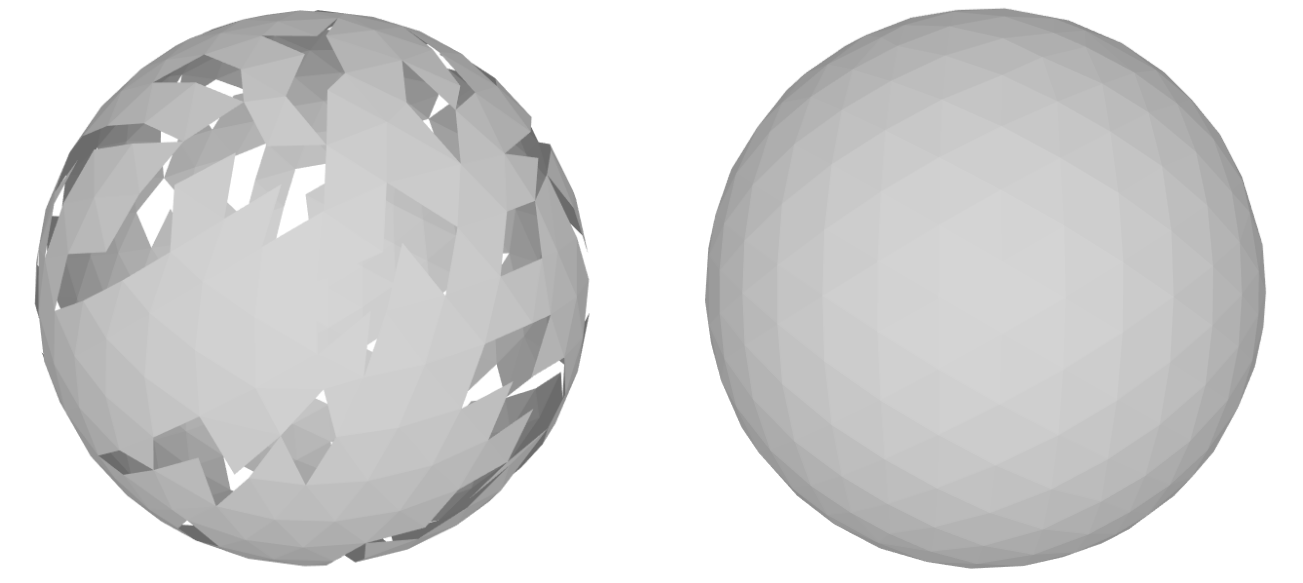
\includegraphics[width=0.75\textwidth]{images/delaunay_vs_gravitycenter}}
        \caption[]{TODO}
        %id obrazku, pomocou ktoreho sa budeme na obrazok odvolavat
        \label{obr:delaunay_vs_gravitycenter}
    \end{figure}

    \begin{figure}
        \centerline{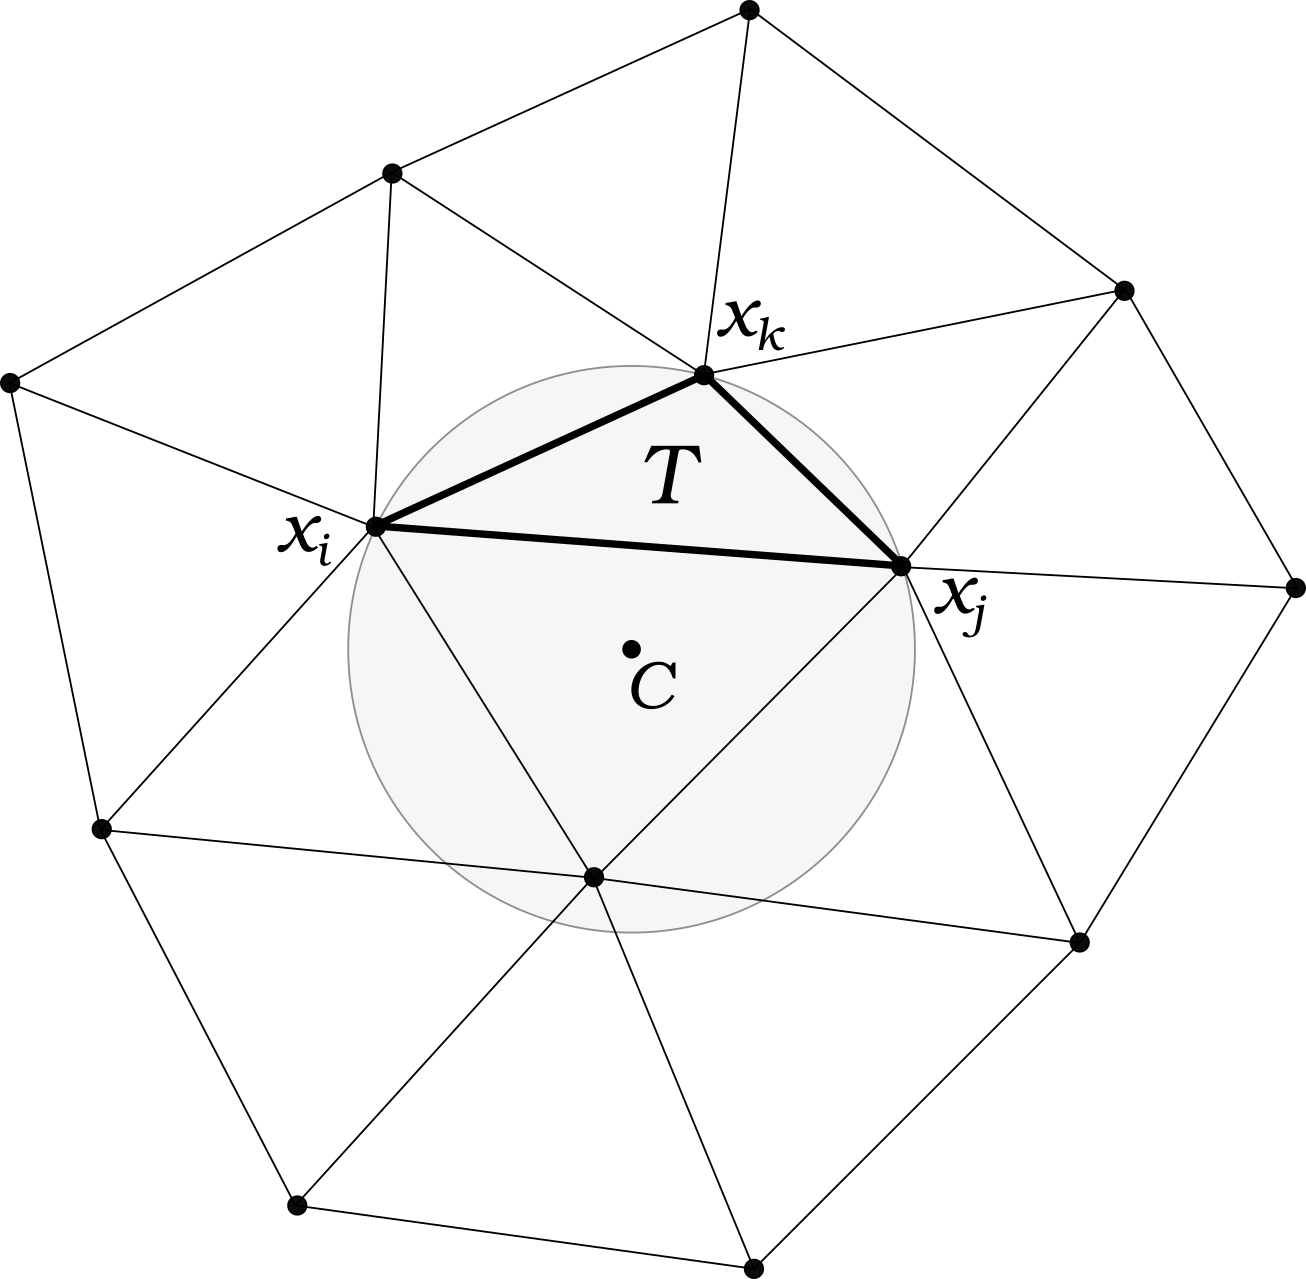
\includegraphics[width=0.35\textwidth]{images/non_delaunay_triangle}}
        \caption[]{TODO}
        %id obrazku, pomocou ktoreho sa budeme na obrazok odvolavat
        \label{obr:non_delaunay_triangle}
    \end{figure}
\end{enumerate}

Po splnení týchto piatich podmienok pridávame trojuholník do meshu. Avšak ešte potrebujeme zistiť 
ako získať ideálny bod $x_k$.

\section{Voľba nového vrchola}

Ako sme už spomínali, algoritmus používa ako 
základnú štruktúru postup opísaný na začiatku kapitoly \ref{kap:algoritmus}. 
Do tohto postupu sme však pridali zmeny založené na našich pozorovaniach. V prvom rade sme 
pozmenili podmienky pre pridanie trojuholníka tak, ako sme opísali v kapitole 
\ref{kap:triangle_conditions}. Avšak tieto zmeny nie sú jediné, pozmenili sme aj 
samotnú štruktúru algoritmu. Takisto sme do algoritmu pridali niekoľko krokov.

\subsection{Základná štruktúra algortimu}

V každom kroku algoritmu vyberieme zo zoznamu hraničných hrán jednu hranu $E$. Pre túto hranu si 
označíme \textit{susedný trojuholník} ako $N$, tento trojuholník je jediný trojuholník v meshi, 
ktorý má ako jednu z hrám $E$. 

\begin{enumerate}
    \item{
        Vytvoríme bod $x_{proj}$ rovnako ako v základnom algoritme. Vzdialenosť $k$ volíme
        ako $\frac{\sqrt 3}{2} \, a$ keďže toto je výška rovnostranného trojuholníka so stranou $a$.
    }
    \item{
        Vyvoríme vrchol $x_{new}$ tak, že sprojektujeme bod $x_{proj}$ na plochu $F$ v smere 
        $\overrightarrow{v} = \overrightarrow{\nabla} F(x_{proj})$. V tomto momente sa z projekcie 
        stáva problém hľadania koreňa funkcie $y = f(x)$. Predpis tejto funkcie získame ako prienik 
        funkcie $F$ a priamky prechádzajúcej bodom $x_{proj}$ so smerovým vektorom $\overrightarrow{v}$. 
        Tu využívame
        \textit{Newton-Raphsonovu metódu} opísanú v kapitole \ref{kap:numeric_methods}. Ako sme 
        už písali, táto metóda je rýchla ale nie je najspoľahlivejšia. Preto ak zlyhá
        použijeme konzervatívnu \textit{metódu bisekcie}.
    }
    \item{
        V prípade, že sa bod $x_{new}$ rovná nejakému hraničnému vrcholu, rovno ho s týmto vrcholom
        spojíme. Táto situácia je síce nepravdepodobná ale pri útvaroch obsahujúcich rovné plochy sa
        deje pravidelne. Bez tohto kroku sa bod $x_{new}$ nemusí spojiť práve s týmto bodom ale
        môže vytvoriť trojuholník, ktorý má horší pomer strán.
    }
    \item{
        V prípade, že $x_{prev} = x_{next}$, teda v meshi je diera v tvare trojuholníka, pridáme tento 
        trojuholník do meshe. Tento krok sme pridali, pretože je pomerne častý, jednoduchý a rýchly.
    }
    \item{
        Nájdeme všetky hraničné vrcholy, ktoré sa nachádzajú v \textit{Delaunayovej guli} pre trojuholník 
        $T_{new} = (x_i, x_j, x_{new})$ a usporiadame ich od najblišieho k hrane $E$. Pri usporiadavaní 
        používame metriku definovanú nasledovne.

        \begin{definition} Vzdialenosť hrany $E=(A,B)$ a vrchola $P$ definujeme ako
        \label{def:segment_point_distance}
        \begin{itemize}
            \item{
                $|AP|$ ak $\measuredangle BAP \in (\frac{\pi}{2}, \frac{3\pi}{2})$
            }

            \item{
                $|BP|$ ak $\measuredangle ABP \in (\frac{\pi}{2}, \frac{3\pi}{2})$
            }

            \item{
                $|EP|$ inak
            }

            
            Pričom $|AP|$, $|BP|$ je euklidovská vzdialenosť bodov v $\mathbb{R}^3$ a $|EP|$ je kolmá 
            vzdialenosť bodu $P$ od priamky na ktorej leží hrana $E$.
        \end{itemize}

        \end{definition}

        Vizualizáciu tejto metriky môžeme vidieť na obrázku \ref{obr:edge_vertex_distance}.

        \begin{figure}
            \centerline{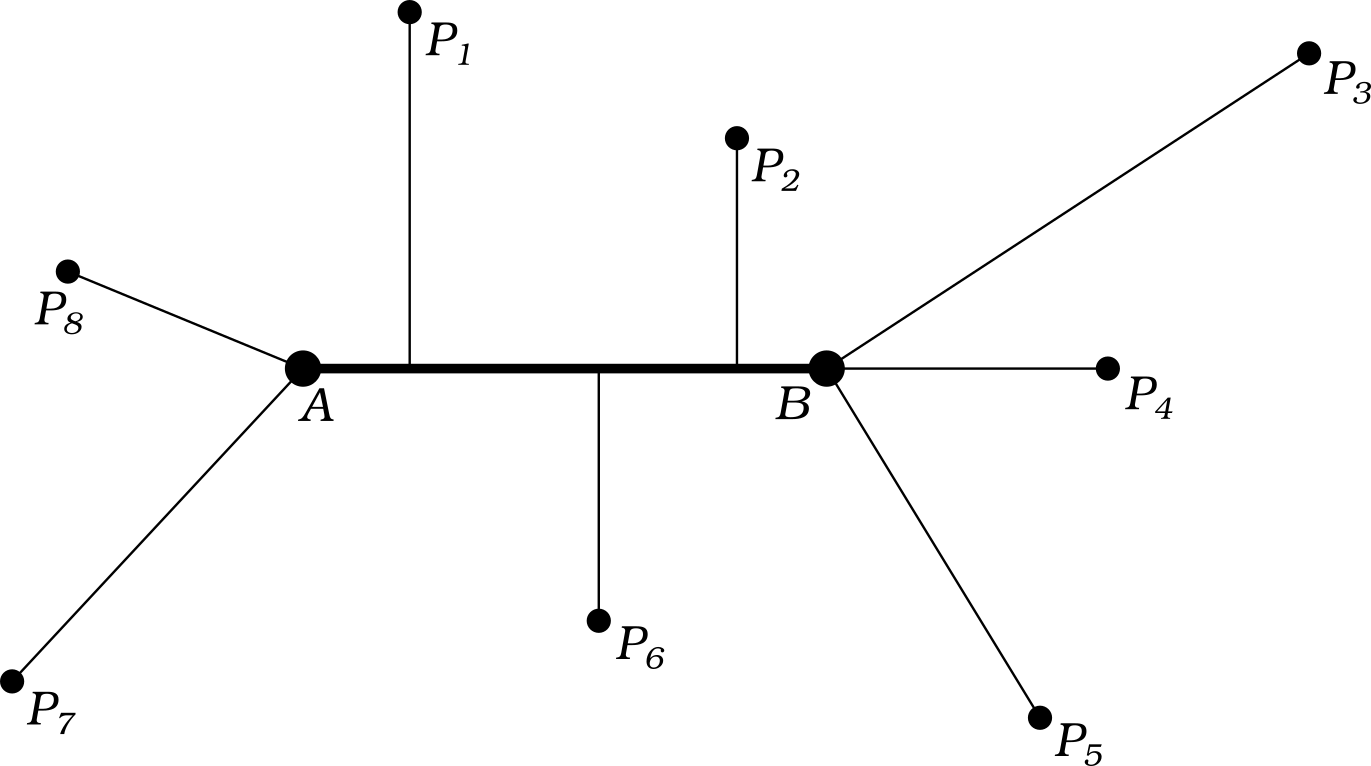
\includegraphics[width=0.6\textwidth]{images/edge_vertex_distance}}
            \caption[Vizualizácia vzdialenosti bodov $P_1, ..., P_8$ od hrany $E=(A,B)$]
            {Vizualizácia vzdialenosti bodov $P_1, ..., P_8$ od hrany $E=(A,B)$}
            %id obrazku, pomocou ktoreho sa budeme na obrazok odvolavat
            \label{obr:edge_vertex_distance}
        \end{figure}


        Následne sa pokúšame vytvoriť trojuholník spĺňajúci podmienky opísané v kapitole 
        \ref{kap:triangle_conditions} s týmito vrcholmi počnúc od najblišieho k hrane.
    }
    \item{
        Nájdeme všetky hraničné vrcholy, ktoré sú k bodu $x_{new}$ bližšie ako $0.4 \, a$
        a pokúšame sa vytvoriť trojuholník s týmito bodmi počnúc od najbližšieho k hrane 
        $E$. Tento krok sa nenachádzal v v pôvodnom algoritme avšak považujeme ho za dôležitý, 
        keďže ako dôsledok nespájania blízkych bodov môžu neskôr vznikať úzke alebo malé trojuholníky. 
        Príklad využitia tohto kroku môžeme vidieť na obrázku \ref{obr:close_points}. 
        \begin{enumerate}[a)]
            \item{
                Trojuholník $T_{new}$ spĺňa \textit{Delaunayovu podmienku}, teda podľa základného 
                algoritmu pridáme trojuholník do meshu. Zdalo by sa nám však správne vytvoriť a 
                pridať do meshu trojuholník $T_{prev} = (x_i, x_j, x_{prev})$. 
            }
            \item{
                Keďže v okolí bodu $x_{new}$ sa nachádza vrchol $x_{prev}$, teda pokúsime
                sa vytvoriť trojuholník s bodom $x_{prev}.$
            }
            \item{
                Trojuholník $T_{prev} = (x_i, x_j, x_{prev})$ spĺňa \textit{Delaunayovu podmienku},
                teda ho pridáme do meshu. 
            }
        \end{enumerate}
        
        \begin{figure}
            \centerline{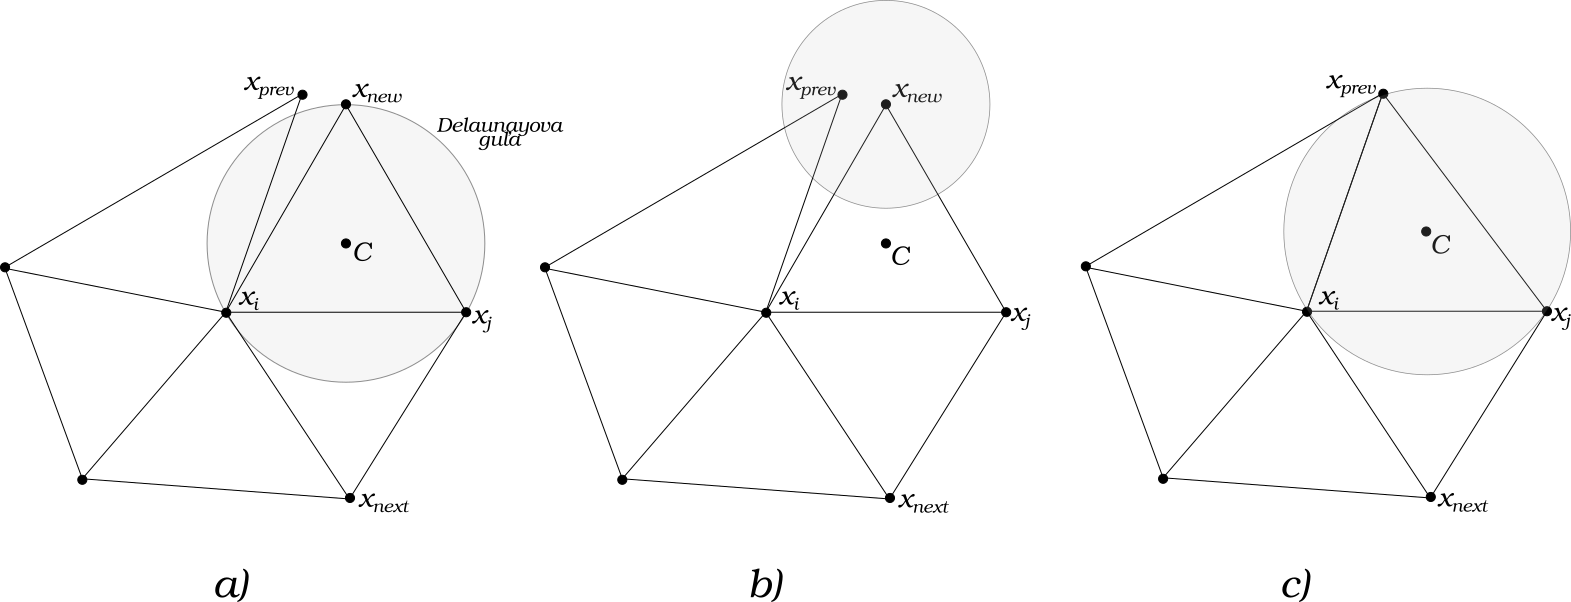
\includegraphics[width=1\textwidth]{images/close_points}}
            \caption[Trojuholník $T_{new}$ spĺňa Delaunayovu podmienku]{Trojuholník $T_{new}$ spĺňa Delaunayovu podmienku}
            %id obrazku, pomocou ktoreho sa budeme na obrazok odvolavat
            \label{obr:close_points}
        \end{figure}
    }
    \item{
        TODO zmeniť presnosť!!!

        Nájdeme najbližšiu hranu k bodu $x_{new}$, opäť používame metriku z definície 
        \ref{def:segment_point_distance}. Ak je táto hrana bližšie ako $\frac{a}{3}$, 
        pokúsime sa vytvoriť trojuholník s koncovými bodmi hrany, ak ani tieto trojuholníky 
        nie sú vyhovujúce, pokúsime sa vytvoriť trojuholník so stredom najbližšej hrany.
        Tento krok pridávame, pretože
        tieto vrcholy sa nám zdajú ako vhodný kandidáti na vytvorenie nového trojuholníka
        aj napriek tomu, že nemusia byť objavené \textit{Delaunayovou podmienkou} ani ako 
        blízke body k bodu $x_{new}$. V tomto prípade nám napadli dva prístupy. Prvý je len pripnúť 
        bod na stred hrany, druhý je daný bod najprv sprojektovať na povrch a následne k nemu bod 
        pripnúť. V druhom prípade je triangulácia presnejšia avšak v prvom vyzerá na pohľad 
        prirodzenejšie. Postup môžeme vidieť na obrázku \ref{obr:closest_edge} kde
        v časti $d)$ ilustrujeme druhý prístup.

        \begin{figure}
            \centerline{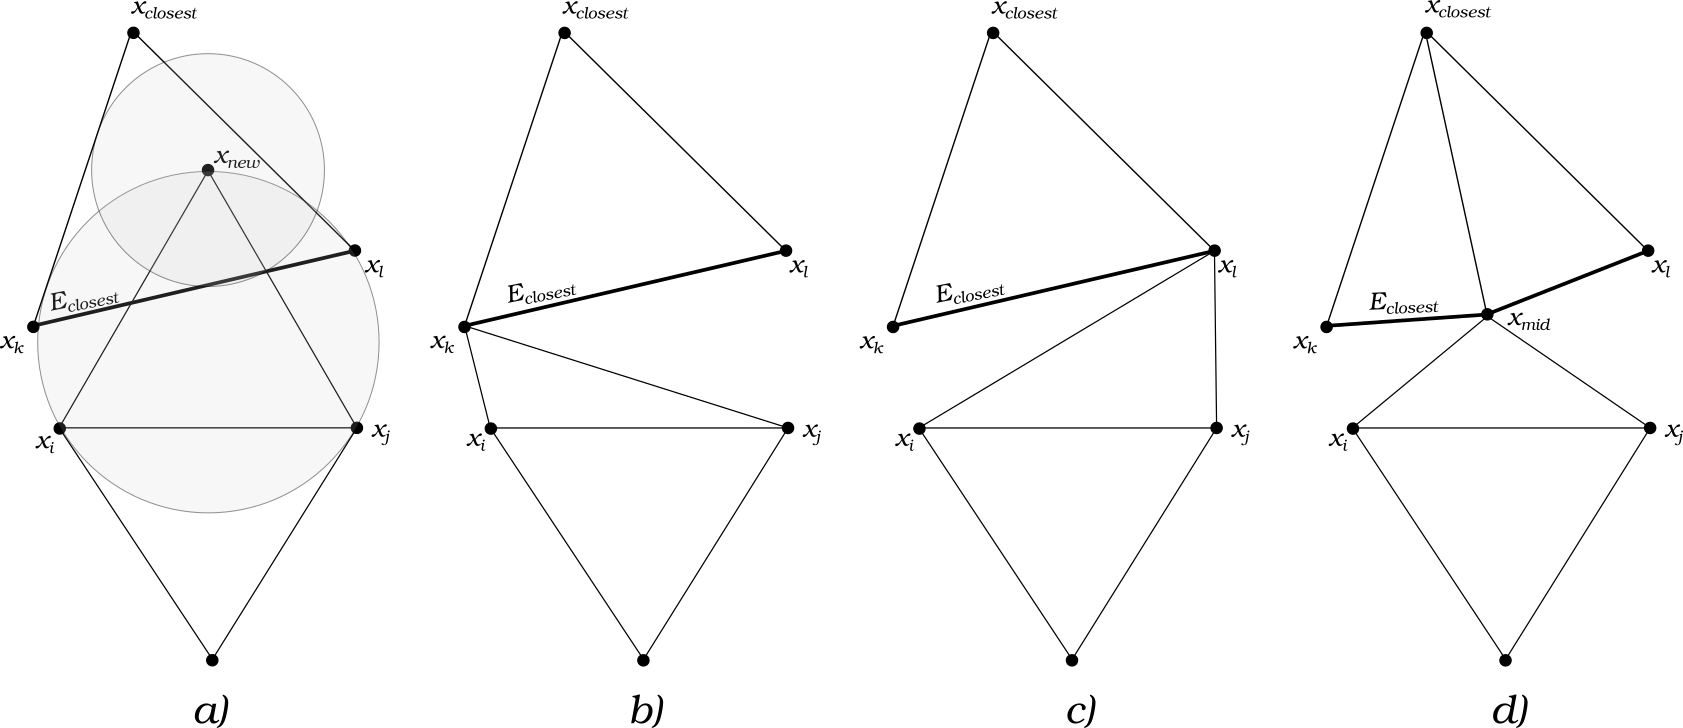
\includegraphics[width=1\textwidth]{images/closest_edge}}
            \caption[TODO]{TODO}
            %id obrazku, pomocou ktoreho sa budeme na obrazok odvolavat
            \label{obr:closest_edge}
        \end{figure}
    }
    \item{
        Ak sa nám doteraz nepodarilo vytvoriť nový trojuholník a trojuholník $T_{new} = (x_i, x_j, x_{new})$
        spĺňa podmienky z kapitoly \ref{kap:triangle_conditions}, pridáme ho do meshu a skončíme.
    }
    \item{
        Ak sa nám nepodarilo pridať ani trojuholník $T_{new}$, pokúsime sa vytvoriť trojuholníky 
        $T_{prev} = (x_i, x_j, x_{prev})$ a $T_{next} = (x_i, x_j, x_{next})$.
    }
    \item{
        Ak sa nám nepodarilo vytvoriť nový trojuholník, označíme hranu $E = (x_i, x_j)$ za skontrolovanú
        a skončíme.
    }
    Algoritmus beží pokým nie sú všetky zostávajúce hrany v zozname hrán skontrolované. Po tomto postupe 
    môžu zostať v meshi diery. Uzatváranie dier budeme riešiť v nasledujúcej kapitole.
\end{enumerate}




















\subsection{Problémy pri voľbe nového vrchola $x$}

Majme hraničnú hranu $E=(x_i, x_j)$ čiastočnej triangulácie $M$. 
V tejto podkapitole opíšeme aké vrcholy $x$ skúšame pre túto hranu. 

V tejto podkapitole opíšeme problémy ktoré sme spozorovali počas štúdia základného 
algoritmu.

\begin{enumerate}

\item{
    

   
}

\item{
    Ďalší problém, ktorý vnímame je pretínanie trojuholníkov. Na obrázku \ref{obr:second_problem} môžeme
    vidieť trojuholník $T_{new}$, ktorého nový vrchol $x_{new}$ nemá žaidne blízke body. 
    Pre tento trojuholník je taktiež splnená \textit{Delaunayova podmienka}, teda by sme ho mali pridať 
    do meshu. Vidíme však, že tento trojuholník sa môže pretínať s iným hraničným trojuholníkom.

    
}

\end{enumerate}
  
\subsection{Navrhované riešenia}

\begin{enumerate}
\item{
    Našim navrhovaným riešením je v okolí vrchola $x_{new}$ pridať guľu s polomerom 
    $0.4-$násobku dĺžky strany trojuholníka. Následne zisťujeme, či sa vnútri tejto gule nachádzajú 
    hraničné body. Tieto body nazveme blízke body k bodu $x_{new}$. V ďalšom kroku 
    sa pokúšame vytvoriť trojuholník s hranou E a blízkymi bodmi počnúc od najbližšieho k hrane $E$. 
    $2D$ ilustáciu riešenia môžeme vidieť na obrázku \ref{obr:first_problem_solution}. 

    \begin{figure}
        \centerline{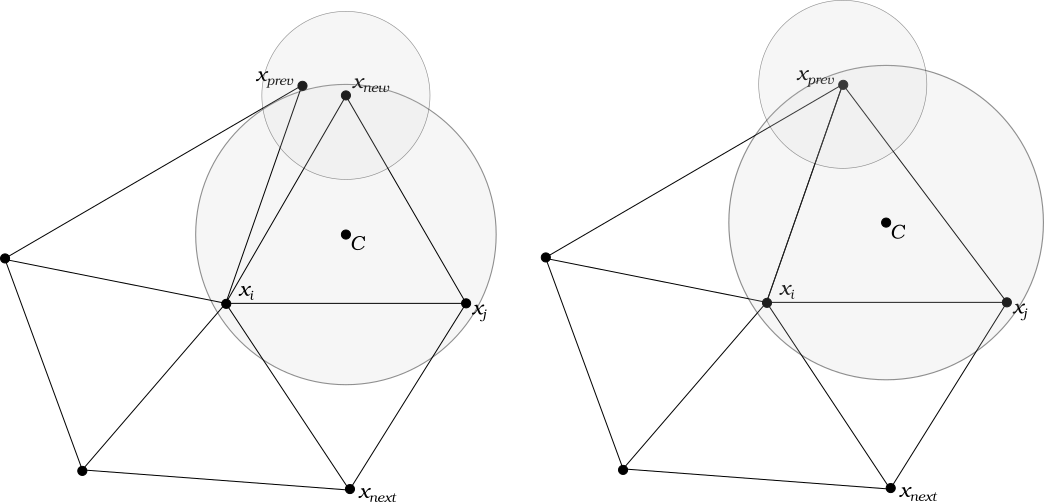
\includegraphics[width=0.7\textwidth]{images/first_problem_solution}}
        \caption[Trojuholník $T_{new}$ má vo svojom okolí blízky bod]{Trojuholník $T_{new}$ má vo svojom okolí blízky bod}
        %id obrazku, pomocou ktoreho sa budeme na obrazok odvolavat
        \label{obr:first_problem_solution}
    \end{figure}
}

\item{

    Naše navrhované riešenie druhého problému je hneď po kontrole blízkych bodov k bodu 
    $x_{new}$ nájsť spomedzi hraničných hrán najbižšiu hranu k bodu $x_{mid}$
    ktorý je stredom hrany $E$. 
    Metrika ktorú používame na nájdenie najbližšej hrany k bodu je definovaná nasledovne.

    Po nájdení najbližšej hrany $E_{closest} = (x_k, x_l)$ 
    k bodu sa pokúsime vytvoriť trojuholník z hrany $E$ a vrchola $x_k$, potom z
    vrchola $x_l$. Ak ani jeden z týchto trojuholníkov nie je vhodný, pokúsime sa 
    vytvoriť trojuholník z hrany $E$ a vrchola $x_{mid}$. Tento vrchol 
    volíme ako stred hrany $E_{closest}$, ktorý sprojektujeme na plochu. Ak je tento trojuholník vhodný
    postupujeme nasledovne. 
    
    \begin{itemize}
    \item{
        Vyberieme z meshu trojuholník z ktorého je hrana $E_{closest}$, označme ho 
        $T_{closest}=(x_k, x_l, x_{closest})$.
    }
    \item{
        Rozdelíme trojuholník $T_{closest}$ na dva trojuholníky $T_1 = (x_k, x_{mid}, x_{closest})$ a
        $T_1 = (x_{mid}, x_l, x_{closest})$.
    }
    \item{
        pridáme trojuholníky $T_1$ a $T_2$ do meshu. 
    }
    \end{itemize}

    Tento postup môžeme vidieť na obrázku \ref{obr:second_problem_solution}.

    \begin{figure}
        \centerline{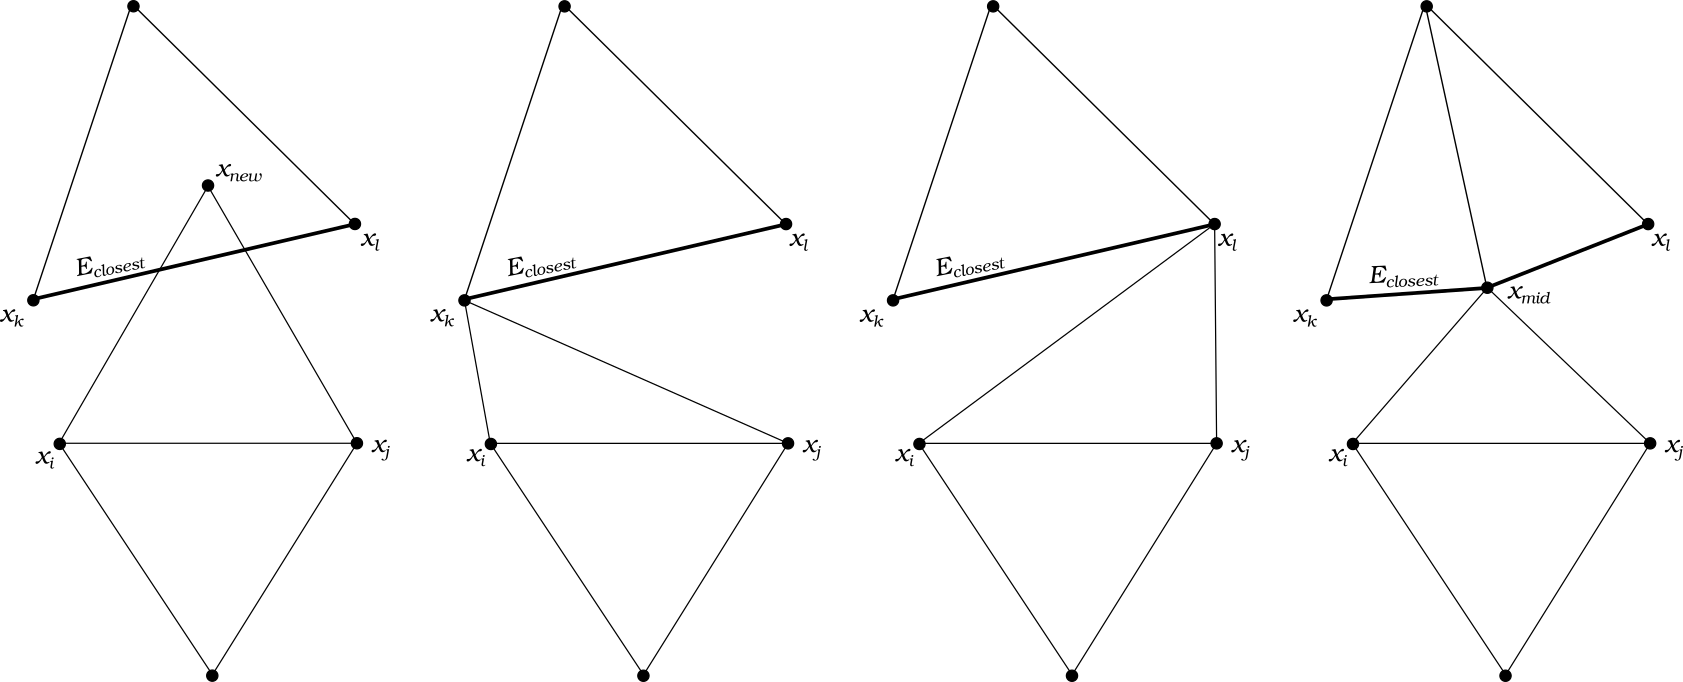
\includegraphics[width=1\textwidth]{images/second_problem_solution}}
        \caption[TODO]{TODO}
        %id obrazku, pomocou ktoreho sa budeme na obrazok odvolavat
        \label{obr:second_problem_solution}
    \end{figure}

    Z toho istého dôvodu sme rozšírili \textit{Delaunayovu podmienku} o podmienku, že 
    v okolí nového vrchola $x_{new}$ sa nesmie nachádzať ťažisko už existujúceho trojuholníka.
    Vizualizáciu tejto podmienky môžeme vidieť na obrázku \ref{obr:centroid_in_delaunay}.

    \begin{figure}
        \centerline{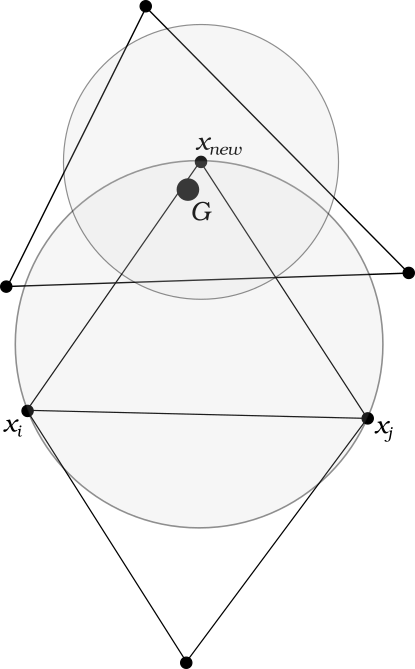
\includegraphics[width=0.25\textwidth]{images/centroid_in_delaunay}}
        \caption[TODO]{TODO}
        %id obrazku, pomocou ktoreho sa budeme na obrazok odvolavat
        \label{obr:centroid_in_delaunay}
    \end{figure}
}
\end{enumerate}

Ak sa nám doteraz nepodarilo vytvoriť žiadny trojuholník s hranou $E$ a zároveň trojuholník 
$T_{new} = (x_i, x_j, x_{new})$ spĺňa všetky podmienky vymenované v podkapitole 
\ref{kap:triangle_conditions}, pridáme ho do meshu. A posunieme sa k ďalšej hraničnej hrane.

\subsection{Skúšanie súsedných hraničných hrán}
Pre zhrnutie uvedieme kroky, z ktorých sa skladal doterajší postup.
\begin{itemize}
\item{
    Vytvorenie nového vrchola $x_{new}$.
}
\item{
    Skúšanie vytvárania trojuholníka s blízkymi bodmi k bodu $x_{new}$.
    Ak sa to podarí, skončíme. 
}
\item{
    Nájdenie najbližšej hraničnej hrany $E_{closest}$.
}
\item{
    Skúšanie vytvárania trojuholníka s koncovými bodmi hraničnej hrany $E_{closest}$ a 
    stredným bodom $x_{mid}$. Ak sa to podarí, skončíme.
}
\item{
    Overenie podmienok opísaných v časti \ref{kap:triangle_conditions}. Ak sú splnené, pridáme do 
    meshu trojuhoľník $T_{new}$ a skončíme.
}
\end{itemize}

V prípade ak sa nám v doterajšom postupe nepodaril vytvoriť nový trojuholník postúpime ku kroku 
číslo 5. základného algoritmu a teda sa pokúšame vytvoriť trojuholník so susednými hraničnými bodmi 
$x_{prev}$ a $x_{next}$. Pre tieto trojuholníky overujeme všetky podmienky z časti 
\ref{kap:triangle_conditions} okrem poslednej, teda tej, že v okolí nového bodu sa nesmie 
nachádzať ťažisko už existujúceho trojuholníka. Ak tieto podmienky platia, pridáme trojuholník 
do meshu a skončíme.

V prípade, že ani jeden z vrcholov $x_{prev}$, $x_{next}$ nevyhovuje podmienkam, zistíme, 
či sa nejaké body nachádzajú v \textit{Delaunayovej guli}, ak áno, skúšame body nachádzajúce
sa v tejto guli, počnúc od najbližšieho k hrane E. Opäť využívame metriku uvedenú v definícii 
\ref{def:segment_point_distance}. Ak sa však ani s týmito bodmi nedá vytvoriť vhodný trojuholník
označíme túto hranu za skontrolovanú a presunieme sa k ďalšej hrane. V momente, keď nemáme žaidnu 
neskontrolovanú hranu, algoritmus končí.

\section{Uzatváranie dier}

Ako si všimli aj autori v článku \cite{akkouche2001adaptive}, po tomto algoritme vznikajú v meshi 
praskliny a diery.

    //TODO toto hodiť do časti implementácia
    
    Na určenie správnej orientácie využívame susedný trojuholník, na obrázku vyznačený 
    ako $N$. Kosínus uhla $\beta$ vieme vypočítať ako skalárny súčin jednotkových vektorov 
    v smere $\overrightarrow{x_i x_j}$ resp. $\overrightarrow{x_i x_{new}}$. 
    Avšak znalosť kosínusu uhla nám určuje iba uhol v intervale $<0, \pi>$. To vyriešime 
//TODO aproximacia normaly VS gradient v bode